%&pdflatex
\documentclass[12pt]{article}


\usepackage{graphicx}
\graphicspath{ {images/} }
\usepackage{colortbl}
\usepackage{xr}
\usepackage{longtable}
\usepackage{xfrac}
\usepackage{tabularx}
\usepackage{booktabs}
\usepackage{hyperref}
\usepackage{xcolor} % for different colour comments
\usepackage{fullpage}
\newcounter{rowcount}
\setcounter{rowcount}{0}
\usepackage{tikz}
\usetikzlibrary{shapes,arrows}


%% Diagram formatting
\tikzstyle{block} = [draw, rectangle, minimum height=1.5em, minimum
width=2em, text centered]
\tikzstyle{arrow} = [thick,-,>=stealth]


\hypersetup{
    bookmarks=true,         % show bookmarks bar?
    colorlinks=true,        % false: boxed links; true: colored links
    linkcolor=blue,        % color of internal links (change box color with linkbordercolor)
    citecolor=green,        % color of links to bibliography
    filecolor=magenta,      % color of file links
    urlcolor=cyan           % color of external links
}


%% Comments
\newif\ifcomments\commentstrue
\ifcomments
\newcommand{\authornote}[3]{\textcolor{#1}{[#3 ---#2]}}
\newcommand{\todo}[1]{\textcolor{red}{[TODO: #1]}}
\else
\newcommand{\authornote}[3]{}
\newcommand{\todo}[1]{}
\fi
\newcommand{\wss}[1]{\authornote{magenta}{SS}{#1}}
\newcommand{\ds}[1]{\authornote{blue}{DS}{#1}}
\newcommand{\kly}[1]{\authornote{green}{KL}{#1}}
\newcommand{\cc}[1]{\authornote{orange}{CC}{#1}}

%%%%%%%%%%%%%%%%%%%%%%%%%%%%%

\begin{document}

\title{System Architecture for Quarters}
\author{Team 6\\ \\James Anthony (anthonjb)\\ Wenqiang Chen (chenw25)\\ Carolyn Chong
(chongce)\\ Kevin Ly (lyk2)}
\date{\today}

\maketitle

\pagebreak

\tableofcontents
\listoffigures

\section*{Revision History}
\begin{tabular}{|c|c|}
\hline
\textbf{Date}  & \textbf{Comments} \\ \hline
January 5, 2016 & Created revision 0. \\ \hline
January 11, 2016 & Completed revision 0. \\
\hline
January 24, 2016 & Updated introduction from past to future tense. \\
\hline
April 23, 2016 & Connection between requirements and Traceability. \\
\hline
\end{tabular}

\section*{Template}
This document does not follow a structured template for all of its organization.

\pagebreak
\section*{Naming Conventions and Terminology}
    \begin{itemize}
    \item House: In the context of this project, a house functions as a set
      which contains one or more users and stores information about the
      physical property, the users, and content added by those users.
    \item User: A user is a user of the application. A user is designated as an administrator or member of a house.
    \item Administrator: The user that creates the house is, by default, the administrator of the house. The administrator of a house is the only member of the house who can change information about the house, upload/delete files, add/delete members, and delete the house.
    \item Maintenance request: A ticket created by a member of a house to inform another member of the same house of property-related maintenance that needs to be addressed.
    \end{itemize}


\pagebreak

%%%%%%%%%%%%%%%%%%%%%%%%%%%%%

%Introduction and Overview
\section{Introduction and Overview}
This document provides a general overview as to how Quarters will be built. Lists of anticipated and unlikely changes begin the document followed by the design of the system architecture. The system architecture will be designed in a modular manner to support information hiding and is laid out here through the use of diagrams. In the Detailed Design document Quarters' system architecture is decomposed and the design details explained based on the Software Requirements Specifications (SRS) document.

\section{Requirements and Design}
Quarters, the web platform is a summation of many different applications that with their own unique features. This ideology, brings emphasis to the modularity of the system, and the encapsulation of each functions affects and information. The visual components of each web page must also be modularized to reduce code repetition. 

%Anticipated Changes
\section{Anticipated Changes}
\begin{enumerate}
  \item \textbf{Design of user interface:} The user interface is expected to change based on feedback from users during usability testing. The interface is expected to change in ways that better support usability principles.
  \item \textbf{Removal of features:} Some features are expected to be removed based on user feedback. If usability testing indicates that a specific feature would not be utilized then it should be removed.
\end{enumerate}

%Unlikely Changes
\section{Unlikely Changes}
\begin{enumerate}
  \item \textbf{Login via social media:} Allows the user to login using accounts from other services such as Facebook, Gmail, Twitter, etc.
  \item \textbf{Live chat:} A platform for real-time communication between users who are currently logged on to Quarters.
\end{enumerate}

%
\section{Decomposition into Components}
\begin{figure}
\centering
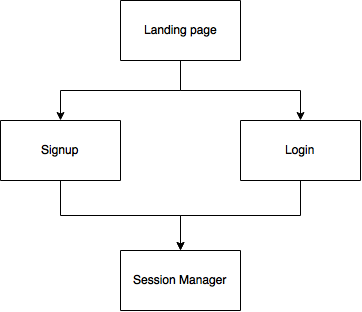
\includegraphics[scale=0.75]{login}
\caption{Authentication control flow}
\label{fig:auflow}
\end{figure}

Figure \ref{fig:auflow} presents flow of logging into the application.
\begin{enumerate}
    \item \textbf{Landing page} - Presents an overview of the application, outlining some of the main features, and provide the option to sign up and login.
    \item \textbf{Signup} - Allows user to register new accounts. Once registration is done, the user is directed to the main application.
    \item \textbf{Login} - Allows user to login with their existing account. Once registration is done, the user is directed to the main application
    \item \textbf{Session Manager} - Once the user is verified (against the database), the user information will be stored into the local session.
\end{enumerate}


\begin{figure}
\centering
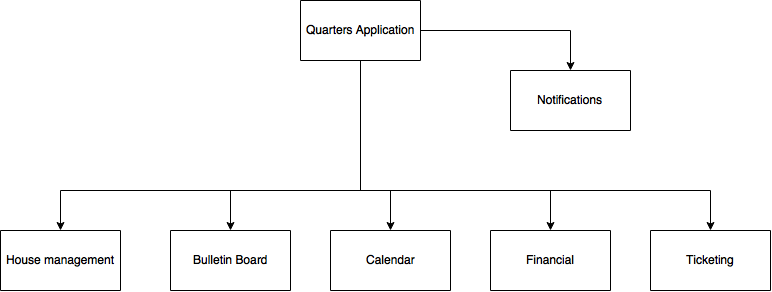
\includegraphics[width=\textwidth]{quarters}
\caption{Demonstrates the flow of requirements within the Javascript modules}
\label{fig:jsflow}
\end{figure}

\

 Figure \ref{fig:jsflow} presents a flow of the Javascript modules
\begin{enumerate}
    \item \textbf{House management} - Handles all activities related to the house. e.g Joining a house, leaving a house, etc.
    \item \textbf{Bulletin Board} - Handles all activities within the bulletin board module. e.g. e.g. make a new post, delete a post, etc.
    \item \textbf{Calendar Board} - Handles all updates  for calendar events. e.g. make a new event, delete event, etc.
    \item \textbf{Financial} - Handles all actions for storing financial records. e.g. post a new bill, pay bill, etc.
    \item \textbf{Ticketing} - Handles all actions for maintenance tickets. e.g. submit a new ticket, close a ticket, etc.
    \item \textbf{Notification} - Handles all actions for notifications. e.g. post notification.
    
    
\end{enumerate}

\end{document}
